\section{Marco y motivación del proyecto}

\noindent La introducción ha de hacer una resumida descripción del marco tecnológico donde se ubica el proyecto, justificando su necesidad y los objetivos que se buscan con su realización, es decir, del problema que se pretende resolver o analizar. También se puede incluir una visión general de las soluciones propuestas, sin entrar en detalles. La introducción debe concluir con una breve descripción (de no más de una página) de la estructura del informe del proyecto, resumiendo de manera escueta los contenidos de cada capítulo. Es frecuente que la introducción sea el último apartado del informe que se escriba.

Las figuras deben citarse en el texto al menos una vez antes de la aparición de cada una. Ver como ejemplo la \autoref{fig:esquema-internet}, en la que se observa un esquema bla, bla, bla, bla...

\begin{figure}[H]
    \centering
    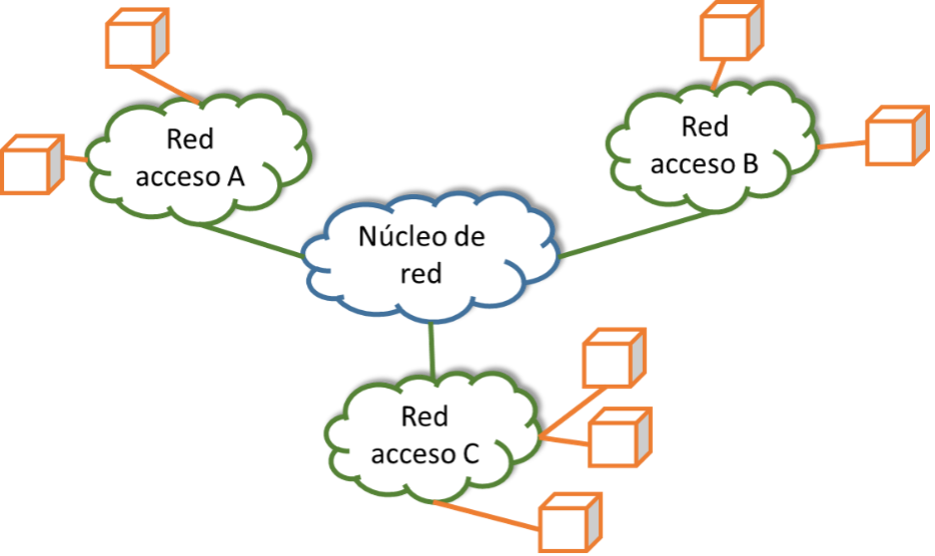
\includegraphics[width=\textwidth]{Imagen 1.png}
    \caption{Esquema conceptual de internet}
    \label{fig:esquema-internet}
\end{figure}

% Las referencias se deben citar asi\cite{javaccgithub}.
\section{Objetivos técnicos y académicos}

\noindent Los objetivos de este proyecto fin de carrera son, desde el punto de vista técnico:

\begin{itemize}
    \item Bla bla bla
\end{itemize}

Desde el punto de vista académico, el proyectista adquiere las siguientes competencias y habilidades:

\begin{itemize}
    \item Bla bla bla
\end{itemize}

\section{Estructura del resto de la memoria}

\noindent En los próximos capítulos de la memoria se ofrecen información sobre... (no más de una página).